\documentclass{article}
\usepackage[utf8]{inputenc}

\usepackage{amsfonts}
\usepackage{amssymb}
\usepackage{amsmath}
\usepackage{amsthm}
\usepackage{enumitem}
\usepackage{float}

\usepackage{graphicx}

\usepackage{bbold}
\usepackage{bm}
\usepackage{color}
\usepackage{hyperref}
\usepackage[margin=2.5cm]{geometry}

\usepackage{fancyhdr}

\usepackage[english]{babel}
\usepackage[T1]{fontenc}

\usepackage{tcolorbox}
\usepackage{fancyvrb}
\usepackage{scrextend}

\makeatletter

\makeatother

\begin{document}

% ==============================================================================

\title{High-Dimensional Statistics}								% Title
\author{Romain LAMBERMONT, Arthur LOUIS}								% Author
\date{\today}						% Date

\makeatletter
\let\thetitle\@title
\let\theauthor\@author
\let\thedate\@date
\makeatother

\pagestyle{fancy}
\fancyhf{}
\rhead{\theauthor}
\lhead{\thetitle}
\cfoot{\thepage}

\begin{titlepage}
 \centering
 \vspace*{0.5 cm}
 
\includegraphics[scale = 0.7]{figs/facsa.png}\\[1.0 cm]	% University Logo
 \textsc{\LARGE \newline\newline Faculty of Applied Science}\\[2.0 cm]	% University Name
 \textsc{\Large MATH2021-1 High-dimensional statistics}\\[0.5 cm]				% Course Code
 \rule{\linewidth}{0.2 mm} \\[0.4 cm]
 {\huge \bfseries Project 1 : Exploratory Data Analysis}\\
 \rule{\linewidth}{0.2 mm} \\[1.5 cm]

 \begin{minipage}{0.5\textwidth}
 	\begin{flushleft} \large
 		\emph{Teacher :}\\
 		Gentiane HAESBROECK\\
    \vspace{0.5cm}
 		\end{flushleft}
 		\end{minipage}~
 		\begin{minipage}{0.4\textwidth}

 		\begin{flushright} \large
 		\emph{Group :} \\
    Romain LAMBERMONT\\
    Arthur LOUIS\\
      
 	\end{flushright}

 \end{minipage}\\[2 cm]
 \thedate
\end{titlepage}

% ==============================================================================
\thispagestyle{empty}
\tableofcontents
\listoffigures
\listoftables
\pagebreak
\setcounter{page}{1}

\subsection{Discussion on the data}
%% TODO

\subsection{Link between the variables}
%% TODO

\section{Information about missing data}
We have a total of $2.1\%$ of missing values but this number is overestimated because the binary indicators are taken into account. The real ratio is $1.7\%$
without this indicators.
The missing values are due to hardware problems related to the measuring instruments
and to the fact that the data was collected in a real environment.

\begin{figure}[H]
  \centering
  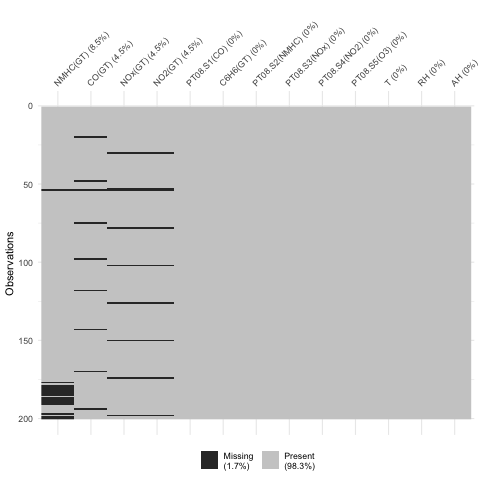
\includegraphics[width=0.5\textwidth]{figs/missing_values.png}
  \caption{Missing data}
  \label{fig:missing_data}
\end{figure}

\begin{figure}[H]
  \centering
  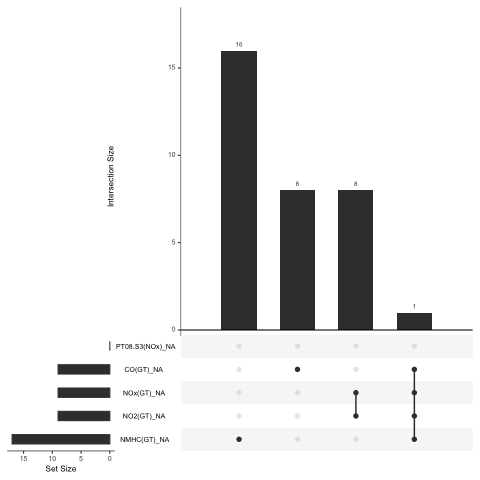
\includegraphics[width=0.5\textwidth]{figs/missing_values_heatmap.png}
  \caption{Missing data heatmap}
  \label{fig:missing_data_heatmap}
\end{figure}

To handle the missing values we will use for the rest of the project the complete case strategy.
Indeed, replacing missing data by the mean would not be a good idea because it would change the correlation structure of the data which is important for the next steps.
We only have 33 lines with missing values so we can afford to remove them keeping the ratio $\frac{n}{p} > 5$ as we have a total of 163 lines and 21 variables, we keep $7.8 > 5$.

Using the two figures here above we can see that the missing values are not randomly distributed.
Indeed, when there's a failure on the CO sensor, the NOx and NO$_2$ sensors are also failing a little bit after.
We can also see that when the NOx sensor is failing, the NO$_2$ sensor is also failing, this is quite logical because NO$_2$ is a kind of NOx.
Around the 175th observation, we can see the non methane hydrocarbons sensor failing and never quite coming to its original state. 
All these observations are confirmed by the second figure as the NMHC measure is the most missing well over the CO sensor or the couple NOx/NO$_2$ which is failling the same number of times.




\section{Exploratory data analysis}

\subsection{Statistical analysis}
\begin{table}[h]
  \centering
  \begin{tabular}{|c|c|c|c|c|c|c|c|}
    \hline
      & vars & n & mean & sd & median & trimmed & mad\\
    \hline
    CO(GT) & 1 & 191 & 2.748691 & 1.596801 & 2.50 & 2.560784 & 1.33434\\
    \hline
    PT08.S1(CO) & 2 & 200 & 1339.000000 & 255.446559 & 1332.50 & 1328.356250 & 233.50950\\
    \hline
    NMHC(GT) & 3 & 183 & 160.158470 & 139.745774 & 122.00 & 138.448980 & 118.60800\\
    \hline
    C6H6(GT) & 4 & 200 & 12.254000 & 8.274006 & 11.05 & 11.318750 & 7.33887\\
    \hline
    PT08.S2(NMHC) & 5 & 200 & 1016.950000 & 281.940276 & 1017.50 & 1005.556250 & 278.72880\\
    \hline
    NOx(GT) & 6 & 191 & 175.842932 & 94.999980 & 161.00 & 168.830065 & 85.99080\\
    \hline
    PT08.S3(NOx) & 7 & 200 & 1003.195000 & 278.431170 & 945.00 & 976.950000 & 234.99210\\
    \hline
    NO2(GT) & 8 & 191 & 115.612565 & 34.357971 & 119.00 & 116.549020 & 35.58240\\
    \hline
    PT08.S4(NO2) & 9 & 200 & 1671.040000 & 305.901187 & 1622.50 & 1641.750000 & 237.21600\\
    \hline
  \end{tabular}

  \begin{tabular}{|c|c|c|c|c|c|c|}
    \hline
      & min & max & range & skew & kurtosis & se\\
    \hline
    CO(GT) & 0.5 & 8.1 & 7.6 & 1.0755547 & 0.9704424 & 0.1155405\\
    \hline
    PT08.S1(CO) & 831.0 & 2040.0 & 1209.0 & 0.3506958 & -0.0955406 & 18.0627994\\
    \hline
    NMHC(GT) & 7.0 & 685.0 & 678.0 & 1.3200143 & 1.4422105 & 10.3303049\\
    \hline
    C6H6(GT) & 1.0 & 39.2 & 38.2 & 1.0086394 & 0.8567735 & 0.5850606\\
    \hline
    PT08.S2(NMHC) & 501.0 & 1754.0 & 1253.0 & 0.3211184 & -0.3339212 & 19.9361881\\
    \hline
    NOx(GT) & 16.0 & 478.0 & 462.0 & 0.6699740 & -0.0263597 & 6.8739573\\
    \hline
    PT08.S3(NOx) & 537.0 & 1918.0 & 1381.0 & 0.9745243 & 0.9172654 & 19.6880569\\
    \hline
    NO2(GT) & 28.0 & 194.0 & 166.0 & -0.2179968 & -0.4405303 & 2.4860555\\
    \hline
    PT08.S4(NO2) & 1134.0 & 2679.0 & 1545.0 & 0.9116828 & 0.7869557 & 21.6304804\\
    \hline
  \end{tabular}
\end{table}

\begin{table}[h]
  \centering
  \begin{tabular}{|c|c|c|c|c|c|c|c|}
    \hline
    & vars & n & mean & sd & median & trimmed & mad\\
    \hline
    PT08.S5(O3) & 1 & 200 & 1233.2450000 & 389.2906253 & 1204.5000 & 1222.0375000 & 384.734700\\
    \hline
    T & 2 & 200 & 15.1965000 & 5.5702402 & 14.3000 & 14.8068750 & 5.189100\\
    \hline
    RH & 3 & 200 & 49.8030000 & 15.1352426 & 53.9000 & 50.6387500 & 15.270780\\
    \hline
    AH & 4 & 200 & 0.8085450 & 0.1059962 & 0.8125 & 0.8092338 & 0.104375\\
    \hline
    HIGH\_CO & 5 & 191 & 0.7225131 & 0.4489355 & 1.0000 & 0.7777778 & 0.000000\\
    \hline
    HIGH\_NMHC & 6 & 183 & 0.9945355 & 0.0739221 & 1.0000 & 1.0000000 & 0.000000\\
    \hline
    HIGH\_C6H6 & 7 & 200 & 0.6500000 & 0.4781665 & 1.0000 & 0.6875000 & 0.000000\\
    \hline
    HIGH\_NOx & 8 & 191 & 0.9947644 & 0.0723575 & 1.0000 & 1.0000000 & 0.000000\\
    \hline
    HIGH\_NO2 & 9 & 191 & 0.5968586 & 0.4918179 & 1.0000 & 0.6209150 & 0.000000\\
    \hline
  \end{tabular}
  
  \begin{tabular}{|c|c|c|c|c|c|c|}
    \hline
    & min & max & range & skew & kurtosis & se\\
    \hline
    PT08.S5(O3) & 384.0000 & 2359.0000 & 1975.0000 & 0.2942286 & -0.1157893 & 27.5270041\\
    \hline
    T & 6.1000 & 29.3000 & 23.2000 & 0.6005822 & -0.4670720 & 0.3938755\\
    \hline
    RH & 14.9000 & 81.1000 & 66.2000 & -0.4375140 & -0.8600569 & 1.0702233\\
    \hline
    AH & 0.5237 & 1.0945 & 0.5708 & 0.0279583 & -0.2727186 & 0.0074951\\
    \hline
    HIGH\_CO  & 1.0000 & 1.0000 & -0.9861019 & -1.0329289 & 0.0324838\\
    \hline
    HIGH\_NMHC & 0.0000 & 1.0000 & 1.0000 & -13.3067908 & 176.0326973 & 0.0054645\\
    \hline
    HIGH\_C6H6 & 0.0000 & 1.0000 & 1.0000 & -0.6242595 & -1.6183168 & 0.0338115\\
    \hline
    HIGH\_NOx & 0.0000 & 1.0000 & 1.0000 & -13.6039602 & 184.0313314 & 0.0052356\\
    \hline
    HIGH\_NO2 & 0.0000 & 1.0000 & 1.0000 & -0.3918179 & -1.8561145 & 0.0355867\\
    \hline
  \end{tabular}  

  \caption{Summary statistics}
\end{table}


\begin{figure}[H]
  \centering
  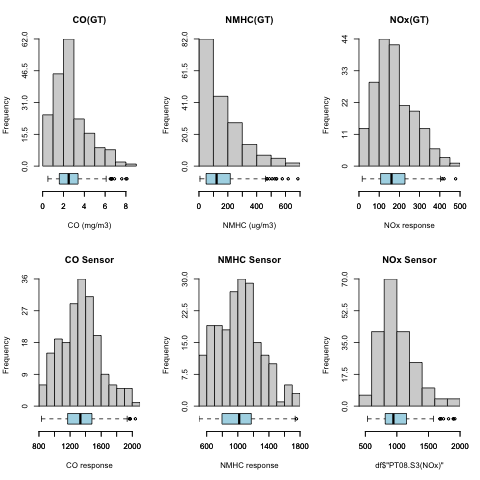
\includegraphics[width=0.5\textwidth]{figs/summary_1.png}
\end{figure}

\begin{figure}[H]
  \centering
  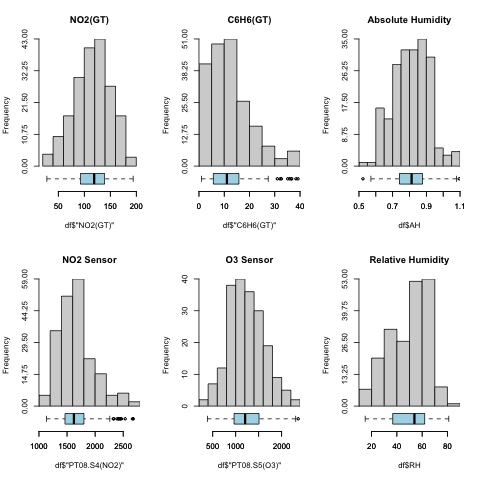
\includegraphics[width=0.5\textwidth]{figs/summary_2.png}
\end{figure}

\begin{figure}[H]
  \centering
  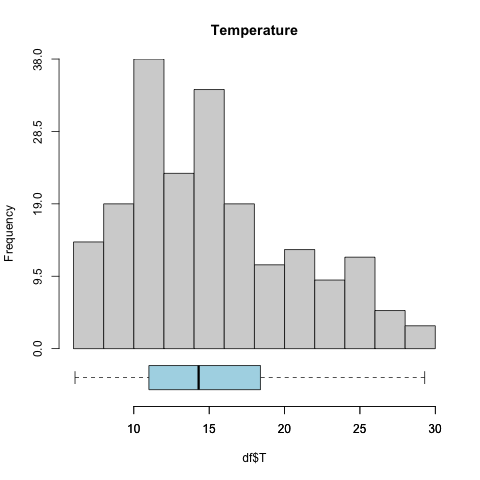
\includegraphics[width=0.5\textwidth]{figs/summary_3.png}
  \label{fig:summary}
  \caption{Summary of the data}
\end{figure}


\subsection{Correlation structure of the data}
\begin{figure}[H]
  \centering
  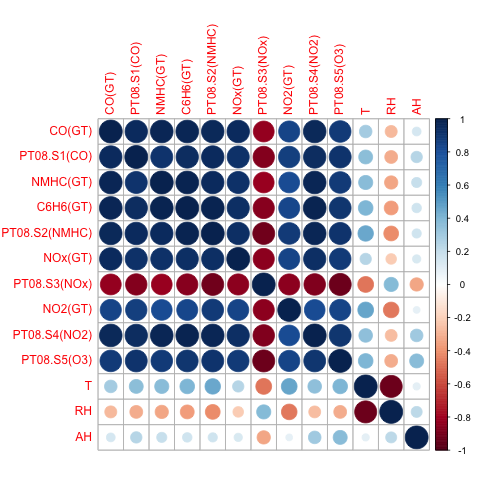
\includegraphics[width=0.5\textwidth]{figs/corr.png}
  \caption{Correlation matrix}
  \label{fig:corr}
\end{figure}

\begin{figure}[H]
  \centering
  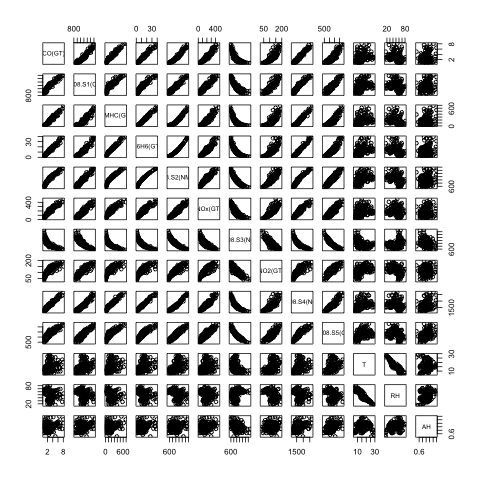
\includegraphics[width=0.5\textwidth]{figs/scatter_matrix.png}
  \caption{Scatter matrix}
  \label{fig:scatter_matrix}
\end{figure}

\subsection{Outlying observations using Mahalanobis distance}
%% TODO

\section{Correlation analysis with data reduction}

\subsection{Choice between PCA and t-SNE}
By looking at the matrix plot, we can see that a lot of variables are correlated. We can exclude from our analysis the 3 colomns: T, RH and AH because there are the less correlated

We decided to use PCA for the correlation analysis because it is a deterministic algorithm and we can reproduce the same results. 
We know that PCA is not the best algorithm in general but in our case, our data are very correlate so this method work really well in our case. 
A very good thing with PCA is that there isn't any hyperparameter to tune the algorithm is so much more easy to use than t-SNE.

\begin{figure}[h]
\centering
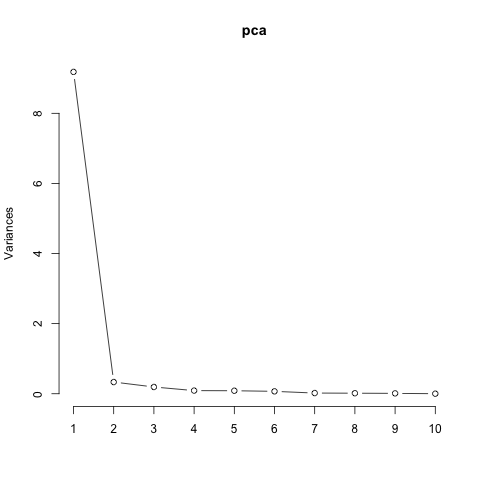
\includegraphics[width=0.5\textwidth]{figs/pca.png}
\caption{Scree plot of the PCA}
\label{fig:scree_plot}
\end{figure}

\subsection{2D plot of the data}


\begin{figure}[H]
\centering
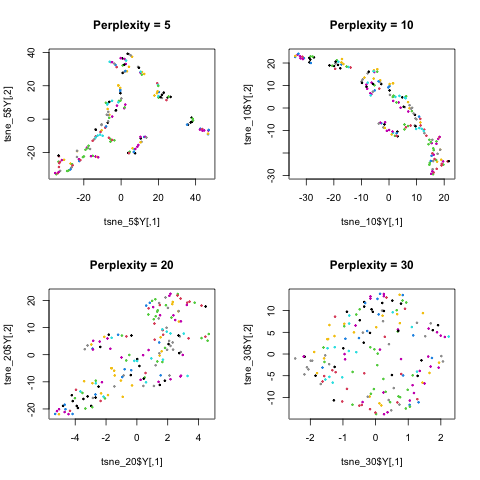
\includegraphics[width=0.5\textwidth]{figs/tsne.png}
\caption{2D plot of the data}
\label{fig:2d_plot}
\end{figure}


\end{document}\documentclass{article}
\usepackage[utf8]{inputenc}

\usepackage{amsfonts}
\usepackage{amssymb}
\usepackage{amsmath}
\usepackage{amsthm}
\usepackage{enumitem}

\usepackage{graphicx}

\usepackage{bbold}
\usepackage{bm}
\usepackage{color}
\usepackage{hyperref}
\usepackage[margin=2.5cm]{geometry}

\usepackage{fancyhdr}

\usepackage[english]{babel}
\usepackage[T1]{fontenc}

\usepackage{tcolorbox}
\usepackage{fancyvrb}
\usepackage{scrextend}

\makeatletter

\makeatother

\begin{document}

% ==============================================================================

\title{High-Dimensional Statistics}								% Title
\author{Romain LAMBERMONT, Arthur LOUIS}								% Author
\date{\today}						% Date

\makeatletter
\let\thetitle\@title
\let\theauthor\@author
\let\thedate\@date
\makeatother

\pagestyle{fancy}
\fancyhf{}
\rhead{\theauthor}
\lhead{\thetitle}
\cfoot{\thepage}

\begin{titlepage}
 \centering
 \vspace*{0.5 cm}
 
\includegraphics[scale = 0.7]{figs/facsa.png}\\[1.0 cm]	% University Logo
 \textsc{\LARGE \newline\newline Faculty of Applied Science}\\[2.0 cm]	% University Name
 \textsc{\Large MATH2021-1 High-dimensional statistics}\\[0.5 cm]				% Course Code
 \rule{\linewidth}{0.2 mm} \\[0.4 cm]
 {\huge \bfseries Project 1 : Exploratory Data Analysis}\\
 \rule{\linewidth}{0.2 mm} \\[1.5 cm]

 \begin{minipage}{0.5\textwidth}
 	\begin{flushleft} \large
 		\emph{Teacher :}\\
 		Gentiane HAESBROECK\\
    \vspace{0.5cm}
 		\end{flushleft}
 		\end{minipage}~
 		\begin{minipage}{0.4\textwidth}

 		\begin{flushright} \large
 		\emph{Group :} \\
    Romain LAMBERMONT\\
    Arthur LOUIS\\
      
 	\end{flushright}

 \end{minipage}\\[2 cm]
 \thedate
\end{titlepage}

% ==============================================================================
\thispagestyle{empty}
\tableofcontents
\listoffigures
\listoftables
\pagebreak
\setcounter{page}{1}

\subsection{Discussion on the data}
%% TODO

\subsection{Link between the variables}
%% TODO

\section{Information about missing data}
We have a total of $2.1\%$ of missing values but this number is overestimated because the binary indicators are taken into account. The real ratio is $1.7\%$
without this indicators.
The missing values are due to hardware problems related to the measuring instruments
and to the fact that the data was collected in a real environment.

\begin{figure}[H]
  \centering
  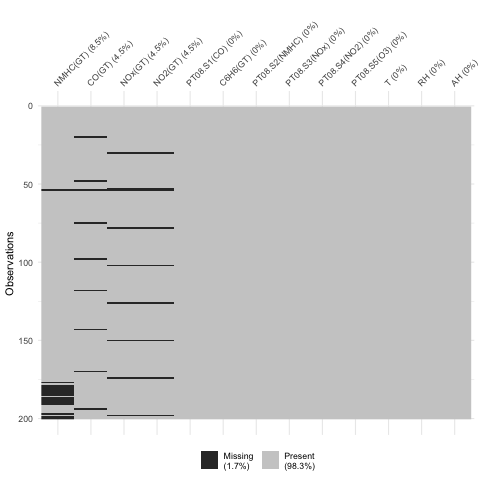
\includegraphics[width=0.5\textwidth]{figs/missing_values.png}
  \caption{Missing data}
  \label{fig:missing_data}
\end{figure}

\begin{figure}[H]
  \centering
  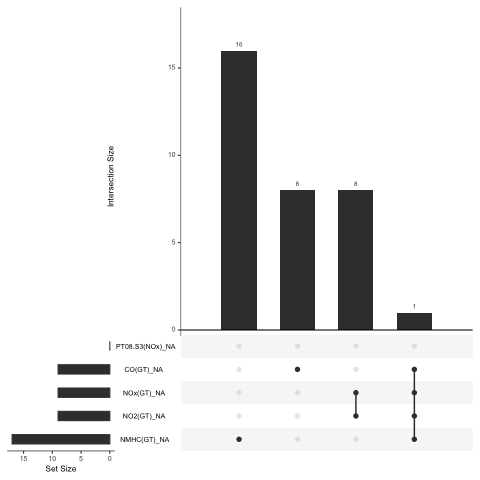
\includegraphics[width=0.5\textwidth]{figs/missing_values_heatmap.png}
  \caption{Missing data heatmap}
  \label{fig:missing_data_heatmap}
\end{figure}

To handle the missing values we will use for the rest of the project the complete case strategy.
Indeed, replacing missing data by the mean would not be a good idea because it would change the correlation structure of the data which is important for the next steps.
We only have 33 lines with missing values so we can afford to remove them keeping the ratio $\frac{n}{p} > 5$ as we have a total of 163 lines and 21 variables, we keep $7.8 > 5$.

Using the two figures here above we can see that the missing values are not randomly distributed.
Indeed, when there's a failure on the CO sensor, the NOx and NO$_2$ sensors are also failing a little bit after.
We can also see that when the NOx sensor is failing, the NO$_2$ sensor is also failing, this is quite logical because NO$_2$ is a kind of NOx.
Around the 175th observation, we can see the non methane hydrocarbons sensor failing and never quite coming to its original state. 
All these observations are confirmed by the second figure as the NMHC measure is the most missing well over the CO sensor or the couple NOx/NO$_2$ which is failling the same number of times.




\section{Exploratory data analysis}

\subsection{Statistical analysis}
\begin{table}[h]
  \centering
  \begin{tabular}{|c|c|c|c|c|c|c|c|}
    \hline
      & vars & n & mean & sd & median & trimmed & mad\\
    \hline
    CO(GT) & 1 & 191 & 2.748691 & 1.596801 & 2.50 & 2.560784 & 1.33434\\
    \hline
    PT08.S1(CO) & 2 & 200 & 1339.000000 & 255.446559 & 1332.50 & 1328.356250 & 233.50950\\
    \hline
    NMHC(GT) & 3 & 183 & 160.158470 & 139.745774 & 122.00 & 138.448980 & 118.60800\\
    \hline
    C6H6(GT) & 4 & 200 & 12.254000 & 8.274006 & 11.05 & 11.318750 & 7.33887\\
    \hline
    PT08.S2(NMHC) & 5 & 200 & 1016.950000 & 281.940276 & 1017.50 & 1005.556250 & 278.72880\\
    \hline
    NOx(GT) & 6 & 191 & 175.842932 & 94.999980 & 161.00 & 168.830065 & 85.99080\\
    \hline
    PT08.S3(NOx) & 7 & 200 & 1003.195000 & 278.431170 & 945.00 & 976.950000 & 234.99210\\
    \hline
    NO2(GT) & 8 & 191 & 115.612565 & 34.357971 & 119.00 & 116.549020 & 35.58240\\
    \hline
    PT08.S4(NO2) & 9 & 200 & 1671.040000 & 305.901187 & 1622.50 & 1641.750000 & 237.21600\\
    \hline
  \end{tabular}

  \begin{tabular}{|c|c|c|c|c|c|c|}
    \hline
      & min & max & range & skew & kurtosis & se\\
    \hline
    CO(GT) & 0.5 & 8.1 & 7.6 & 1.0755547 & 0.9704424 & 0.1155405\\
    \hline
    PT08.S1(CO) & 831.0 & 2040.0 & 1209.0 & 0.3506958 & -0.0955406 & 18.0627994\\
    \hline
    NMHC(GT) & 7.0 & 685.0 & 678.0 & 1.3200143 & 1.4422105 & 10.3303049\\
    \hline
    C6H6(GT) & 1.0 & 39.2 & 38.2 & 1.0086394 & 0.8567735 & 0.5850606\\
    \hline
    PT08.S2(NMHC) & 501.0 & 1754.0 & 1253.0 & 0.3211184 & -0.3339212 & 19.9361881\\
    \hline
    NOx(GT) & 16.0 & 478.0 & 462.0 & 0.6699740 & -0.0263597 & 6.8739573\\
    \hline
    PT08.S3(NOx) & 537.0 & 1918.0 & 1381.0 & 0.9745243 & 0.9172654 & 19.6880569\\
    \hline
    NO2(GT) & 28.0 & 194.0 & 166.0 & -0.2179968 & -0.4405303 & 2.4860555\\
    \hline
    PT08.S4(NO2) & 1134.0 & 2679.0 & 1545.0 & 0.9116828 & 0.7869557 & 21.6304804\\
    \hline
  \end{tabular}
\end{table}

\begin{table}[h]
  \centering
  \begin{tabular}{|c|c|c|c|c|c|c|c|}
    \hline
    & vars & n & mean & sd & median & trimmed & mad\\
    \hline
    PT08.S5(O3) & 1 & 200 & 1233.2450000 & 389.2906253 & 1204.5000 & 1222.0375000 & 384.734700\\
    \hline
    T & 2 & 200 & 15.1965000 & 5.5702402 & 14.3000 & 14.8068750 & 5.189100\\
    \hline
    RH & 3 & 200 & 49.8030000 & 15.1352426 & 53.9000 & 50.6387500 & 15.270780\\
    \hline
    AH & 4 & 200 & 0.8085450 & 0.1059962 & 0.8125 & 0.8092338 & 0.104375\\
    \hline
    HIGH\_CO & 5 & 191 & 0.7225131 & 0.4489355 & 1.0000 & 0.7777778 & 0.000000\\
    \hline
    HIGH\_NMHC & 6 & 183 & 0.9945355 & 0.0739221 & 1.0000 & 1.0000000 & 0.000000\\
    \hline
    HIGH\_C6H6 & 7 & 200 & 0.6500000 & 0.4781665 & 1.0000 & 0.6875000 & 0.000000\\
    \hline
    HIGH\_NOx & 8 & 191 & 0.9947644 & 0.0723575 & 1.0000 & 1.0000000 & 0.000000\\
    \hline
    HIGH\_NO2 & 9 & 191 & 0.5968586 & 0.4918179 & 1.0000 & 0.6209150 & 0.000000\\
    \hline
  \end{tabular}
  
  \begin{tabular}{|c|c|c|c|c|c|c|}
    \hline
    & min & max & range & skew & kurtosis & se\\
    \hline
    PT08.S5(O3) & 384.0000 & 2359.0000 & 1975.0000 & 0.2942286 & -0.1157893 & 27.5270041\\
    \hline
    T & 6.1000 & 29.3000 & 23.2000 & 0.6005822 & -0.4670720 & 0.3938755\\
    \hline
    RH & 14.9000 & 81.1000 & 66.2000 & -0.4375140 & -0.8600569 & 1.0702233\\
    \hline
    AH & 0.5237 & 1.0945 & 0.5708 & 0.0279583 & -0.2727186 & 0.0074951\\
    \hline
    HIGH\_CO  & 1.0000 & 1.0000 & -0.9861019 & -1.0329289 & 0.0324838\\
    \hline
    HIGH\_NMHC & 0.0000 & 1.0000 & 1.0000 & -13.3067908 & 176.0326973 & 0.0054645\\
    \hline
    HIGH\_C6H6 & 0.0000 & 1.0000 & 1.0000 & -0.6242595 & -1.6183168 & 0.0338115\\
    \hline
    HIGH\_NOx & 0.0000 & 1.0000 & 1.0000 & -13.6039602 & 184.0313314 & 0.0052356\\
    \hline
    HIGH\_NO2 & 0.0000 & 1.0000 & 1.0000 & -0.3918179 & -1.8561145 & 0.0355867\\
    \hline
  \end{tabular}  

  \caption{Summary statistics}
\end{table}


\begin{figure}[H]
  \centering
  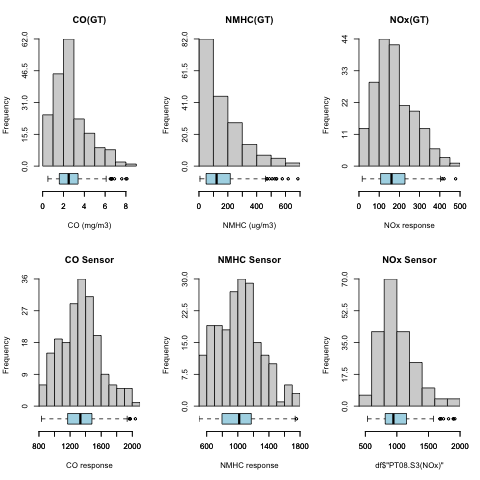
\includegraphics[width=0.5\textwidth]{figs/summary_1.png}
\end{figure}

\begin{figure}[H]
  \centering
  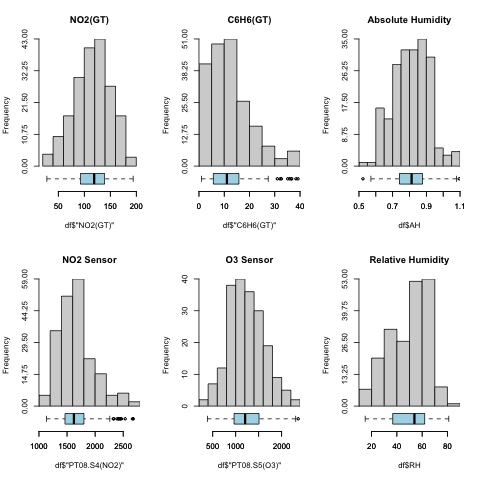
\includegraphics[width=0.5\textwidth]{figs/summary_2.png}
\end{figure}

\begin{figure}[H]
  \centering
  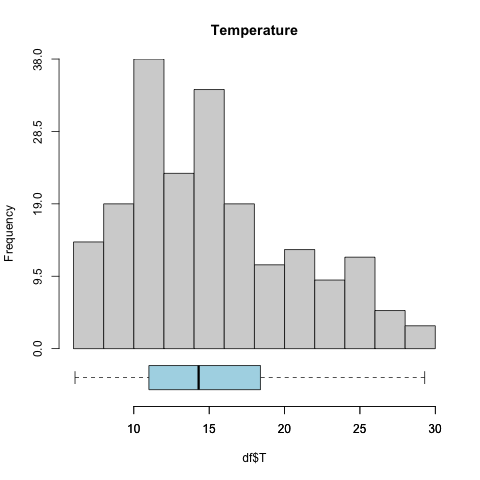
\includegraphics[width=0.5\textwidth]{figs/summary_3.png}
  \label{fig:summary}
  \caption{Summary of the data}
\end{figure}


\subsection{Correlation structure of the data}
\begin{figure}[H]
  \centering
  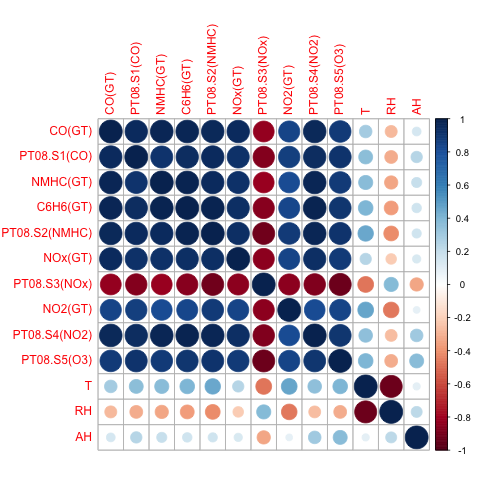
\includegraphics[width=0.5\textwidth]{figs/corr.png}
  \caption{Correlation matrix}
  \label{fig:corr}
\end{figure}

\begin{figure}[H]
  \centering
  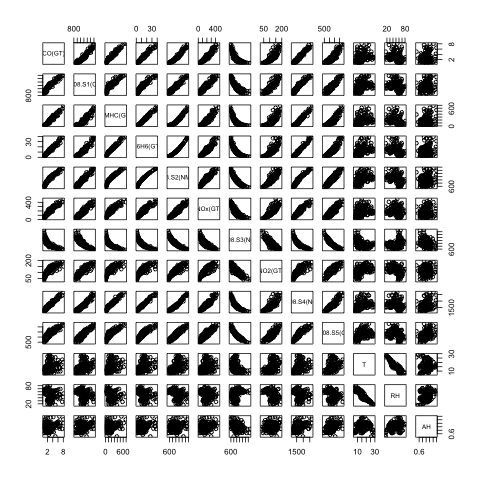
\includegraphics[width=0.5\textwidth]{figs/scatter_matrix.png}
  \caption{Scatter matrix}
  \label{fig:scatter_matrix}
\end{figure}

\subsection{Outlying observations using Mahalanobis distance}
%% TODO

\section{Correlation analysis with data reduction}

\subsection{Choice between PCA and t-SNE}
By looking at the matrix plot, we can see that a lot of variables are correlated. We can exclude from our analysis the 3 colomns: T, RH and AH because there are the less correlated

We decided to use PCA for the correlation analysis because it is a deterministic algorithm and we can reproduce the same results. 
We know that PCA is not the best algorithm in general but in our case, our data are very correlate so this method work really well in our case. 
A very good thing with PCA is that there isn't any hyperparameter to tune the algorithm is so much more easy to use than t-SNE.

\begin{figure}[h]
\centering
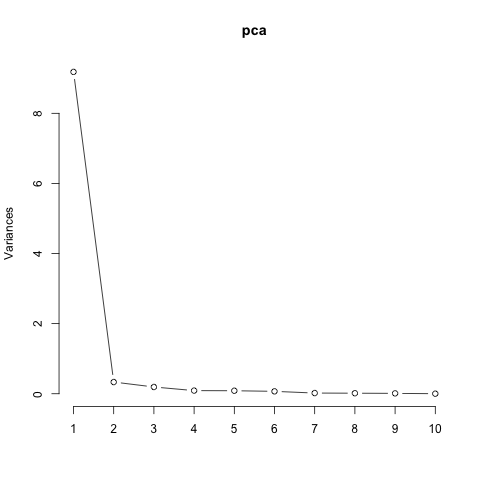
\includegraphics[width=0.5\textwidth]{figs/pca.png}
\caption{Scree plot of the PCA}
\label{fig:scree_plot}
\end{figure}

\subsection{2D plot of the data}


\begin{figure}[H]
\centering
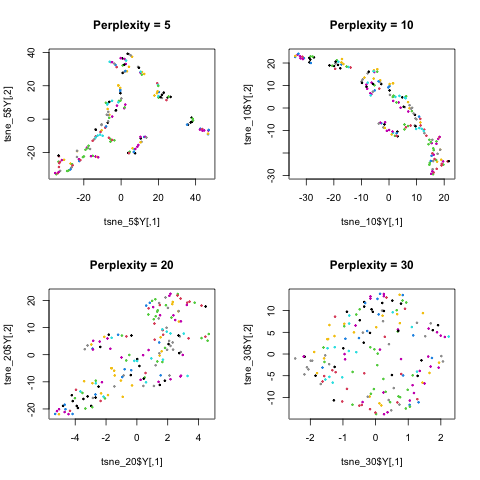
\includegraphics[width=0.5\textwidth]{figs/tsne.png}
\caption{2D plot of the data}
\label{fig:2d_plot}
\end{figure}


\end{document}